%\usepackage{amsmath}
%\usepackage{hyperref}
%\usepackage{amsthm}
%\usepackage{graphicx}
\documentclass[journal, a4paper]{IEEEtran}
\usepackage[italian]{babel}
\usepackage{booktabs}
\usepackage{siunitx}%Questo serve a caricare il pacchetto delle unità di misura del sistema internazionale%
\usepackage[utf8]{inputenc}
\usepackage{graphicx} 
\usepackage{url}
\usepackage{amsmath}
\usepackage{amssymb}


\usepackage{keyval}
\usepackage{xcolor}
\usepackage{caption}
\usepackage{tikz}
\usepackage{circuitikz}
\usepackage{authblk}
%\usepackage{hyperref}

\begin{document}


% Define document title and author
	\title{Tecnologie Digitali - Logbook Week 7}
	\author[1]{Salvatore Bottaro}
		\author[2]{Lorenzo M. Perrone}
		\affil[1]{\texttt{salvo.bottaro@hotmail.it}}
		\affil[2]{\texttt{lorenzo.perrone.lmp@gmail.com}}
	\markboth{Tecnologie Digitali - Di Lieto}{}
	\maketitle
	
\begin{abstract}
	Logbook di laboratorio di Tecnologie Digitali, a.a. 2015/2016. Week 7.
\end{abstract}

\section{Caratteristiche del MOSFET}

Il transistor impiegato è un MOSFET BS170 della Fairchild Semiconductor. Le caratteristiche più importanti del transistor disponibili sul datasheet ai fini dell'esperienza sono elencate in tabella \ref{tab:data}.

\begin{table}[htp]
\centering
\caption{Dati del transistor reperibili nel datasheet.}
\label{tab:data}
\begin{tabular}{|c|c|c|}
\hline 
Parametro & Condizioni & Valore \\ 
\hline 
$I_{DSS}$ & $V_{DS}$ = 25 V, $V_{GS}$ = 0 V & 0.5 $\mu$A (max) \\ 
\hline 
$I_{GSSF}$ & $V_{GS}$ = 15 V, $V_{DS}$ = 0 V & 10 nA (max)\\ 
\hline 
$V_{GS(th)}$ & $V_{DS} = V_{GS}$, $I_D$ = 1 mA & 2.1 V \\ 
\hline 
$g_{FS}$ & $V_{DS}$ = 10 V, $I_D$ = 200 mA & 320 mS \\ 
\hline 
\end{tabular} 
\end{table}

Dove $I_{DSS}$ è la \textit{Zero Gate Voltage Drain Current}, $I_{GSSF}$ la \textit{Forward Gate-Body Leakage}, $V_{GS(th)}$ la tensione di soglia, $g_{FS}$ la transconduttanza.\\
Abbiamo montato sulla breadboard il circuito in figura \ref{fig:circ}, in cui sono indicate anche le porte della scheda impiegate.

\begin{figure}[htp]
\centering
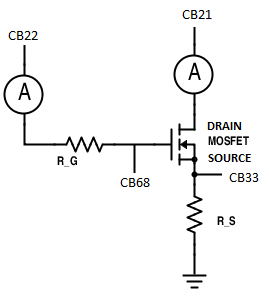
\includegraphics[scale=.5]{mosfet}
\caption{Schema del circuito montato sulla breadboard.}
\label{fig:circ}
\end{figure}

Dal momento che la scheda di acquisizione può erogare al massimo 10 mA e 10 V, abbiamo dovuto dimensionare $R_S$ in modo tale che nelle condizioni estreme, quindi $V_{GS} = V_{DS} = 10 V$, la corrente non raggiungesse i 10 mA. Per R = 1.025 $\pm$ 0.8 $\%$ k$\Omega$ si ha che la corrente massima che può circolare nel circuito, misurata tramite l'amperometro collegato in serie alla CB21, non raggiunge 8 mA, per cui abbiamo preso questo valore della resistenza per $R_S$. Nelle varie prove effettuate è stato impiegato un altro amperometro collegato in serie alla CB22 per misurare la corrente che circola verso il GATE. Ciò che è risultato è che pur avendo impostato il fondoscala più basso la corrente si manteneva costantemente sotto soglia. Questo significa che nel seguito è possibile considerare con ottima approssimazione uguali le correnti al DRAIN e al SOURCE. Inoltre, visto che non si sono praticamente rilevate correnti, la resistenza $R_G$ che noi abbiamo inizialmente scelto di 1 k$\Omega$ non influenza sostanzialmente il circuito.\\
Tramite il VI \texttt{Vin$\_$Vout$\_$2C} abbiamo impostato diversi valori delle tensioni al GAIN e al DRAIN, con il vincolo $V_{GS} = V_{DS}$, cercando il valore della tensione di soglia, ovvero il valore per cui la corrente al DRAIN fosse 1 mA. Abbiamo trovato $V_{GS(th)}$ = 2.23 $\pm$ 0.02 V, simile al valore tipico dichiarato dal datasheet.

\section{Corrente di DRAIN vs tensione sul GATE}

Per misurare come la corrente di DRAIN dipenda dalla tensione di GATE abbiamo utilizzato il VI \texttt{FET$\_$vs$\_$GATE} che fissa il valore della tensione al DRAIN e spazza un intervallo di tensioni da impostare per il GATE. Come prima misura abbiamo impostato $V_{DS}$ = 3 V e spazzato un intervallo di tensioni da 1 V a 7 V. I dati sperimentali sono rappresentati in figura \ref{fig:es4_3}. Come si vede l'andamento non è lineare, inoltre la tensione $V_S$ satura quando $V_S$ si avvicina ai 3 V. Questo perché la tensione al SOURCE deve mantenersi costantemente inferiore alla tensione al DRAIN, quindi per quanto si aumenti la tensione al GATE, non si potrà far scorrere una corrente per cui $V_S \geq V_{DS}$. 

\begin{figure}[htp]
\centering
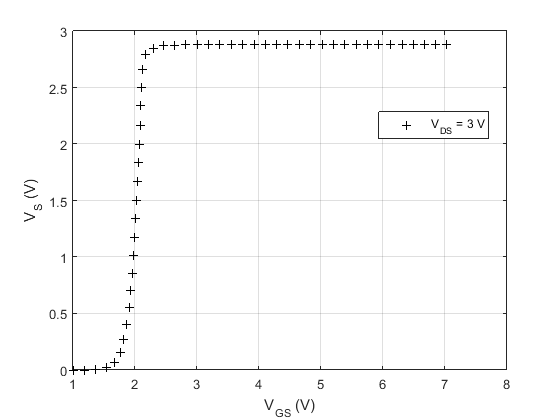
\includegraphics[scale=.5]{es4_3}
\caption{Grafico $V_S$ vs $V_{GS}$ per $V_{DS}$ = 3 V.}
\label{fig:es4_3}
\end{figure}

Fin qui si è assunto che la corrente che scorre al SOURCE sia uguale a quella al GATE. Difatti questa ipotesi è stata già precedentemente verificata, collegando l'amperometro al GATE. Un altro modo per verificare la validità dell'ipotesi é collegare l'amperometro in serie al DRAIN e verificare che la corrente misurata sia compatibile con quella calcolata misurando la tensione al SOURCE. Abbiamo effettuato due prove, in tabella \ref{tab:es6} sono riportati i risultati. Come si vede i valori delle due correnti sono compatibili fra loro.

\begin{table}[htp]
\centering
\caption{Verifica che $I_S = I_D$.}
\label{tab:es6}
\begin{tabular}{|c|c|c|c|c|}
\hline 
$V_{GS}$ (V)& $V_{DS}$ (V) & $V_S$ (V) & $I_D$ (mA)& $I_S$ (mA) \\ 
\hline 
5 & 5 & 2.8875(2) & 2.81 $\pm$ 0.8 $\%$ & 2.82(2) \\ 
\hline 
6 & 6 & 3.849(1) & 3.70 $\pm$ 0.8 $\%$ & 3.76 $\pm$ 0.03 \\ 
\hline 
\end{tabular} 
\end{table}

Abbiamo ripetuto la misura fatta con il VI \texttt{FET$\_$vs$\_$GATE} variando il valore di $V_{GS}$. I vari grafici ottenuti sono riportati in figura \ref{fig:all}. Si vede chiaramente come i grafici hanno tutti lo stesso andamento a basse tensioni al punto che si sovrappongono, mentre saturano ciascuno corrispondentemente al valore di $V_{DS}$, a parte per i casi $V_{DS}$ = 9, 10 V in cui non sono state raggiunte tensioni sufficienti per osservare la saturazione.

\begin{figure}[htp]
\centering
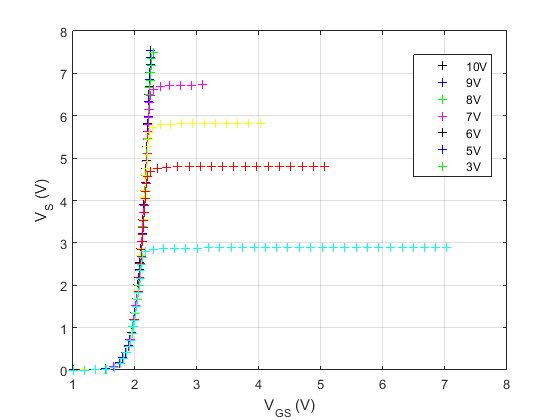
\includegraphics[scale=.5]{all}
\caption{Grafico $V_S$ vs $V_{GS}$ per vari valori di $V_{GS}$.}
\label{fig:all}
\end{figure}

\end{document}